\section{mo\-HC$<$ M $>$ Class Template Reference}
\label{classmo_h_c}\index{moHC@{moHC}}
Hill Climbing (HC).  


{\tt \#include $<$mo\-HC.h$>$}

Inheritance diagram for mo\-HC$<$ M $>$::\begin{figure}[H]
\begin{center}
\leavevmode
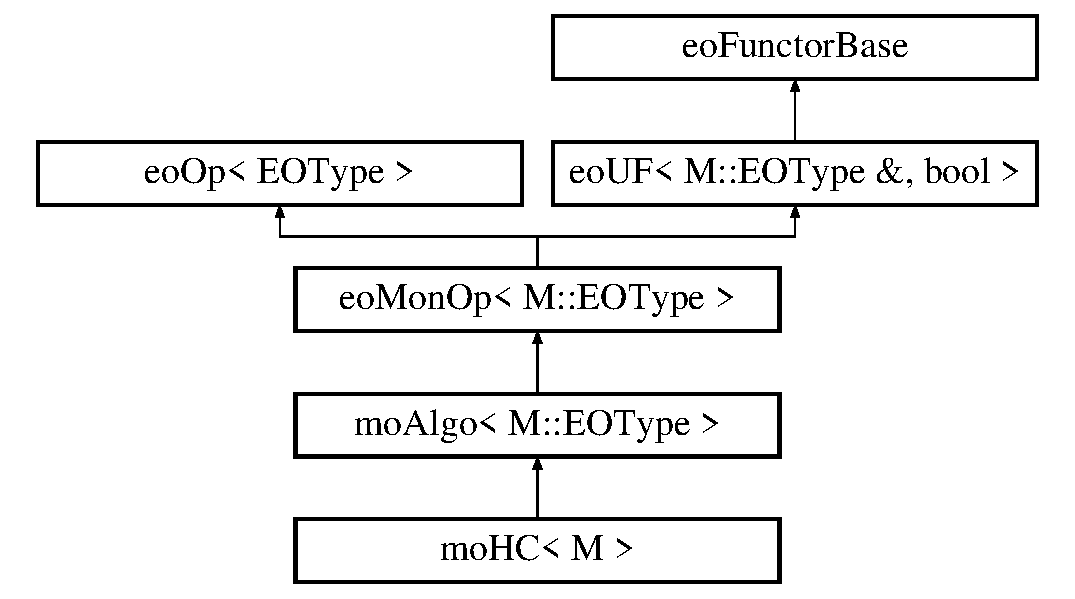
\includegraphics[height=2cm]{classmo_h_c}
\end{center}
\end{figure}
\subsection*{Public Member Functions}
\begin{CompactItemize}
\item 
{\bf mo\-HC} ({\bf mo\-Move\-Init}$<$ M $>$ \&\_\-\_\-move\_\-init, {\bf mo\-Next\-Move}$<$ M $>$ \&\_\-\_\-next\_\-move, {\bf mo\-Move\-Incr\-Eval}$<$ M $>$ \&\_\-\_\-incr\_\-eval, {\bf mo\-Move\-Select}$<$ M $>$ \&\_\-\_\-move\_\-select, eo\-Eval\-Func$<$ {\bf EOT} $>$ \&\_\-\_\-full\_\-eval)
\begin{CompactList}\small\item\em Full constructor. \item\end{CompactList}\item 
{\bf mo\-HC} ({\bf mo\-Move\-Expl}$<$ M $>$ \&\_\-\_\-move\_\-expl, eo\-Eval\-Func$<$ {\bf EOT} $>$ \&\_\-\_\-full\_\-eval)
\begin{CompactList}\small\item\em Light constructor. \item\end{CompactList}\item 
bool {\bf operator()} ({\bf EOT} \&\_\-\_\-sol)
\begin{CompactList}\small\item\em Function which launches the HC. \item\end{CompactList}\end{CompactItemize}
\subsection*{Private Types}
\begin{CompactItemize}
\item 
typedef M::EOType {\bf EOT}\label{classmo_h_c_d219296ede03c679646bce2fe8ff96cb}

\begin{CompactList}\small\item\em Alias for the type. \item\end{CompactList}\item 
typedef EOT::Fitness {\bf Fitness}\label{classmo_h_c_56487c97a7cf0c423cc879d1bbd45027}

\begin{CompactList}\small\item\em Alias for the fitness. \item\end{CompactList}\end{CompactItemize}
\subsection*{Private Attributes}
\begin{CompactItemize}
\item 
{\bf mo\-Move\-Expl}$<$ M $>$ \& {\bf move\_\-expl}\label{classmo_h_c_f6bfb4553fb699f1e08f7d9c37d06103}

\begin{CompactList}\small\item\em Complete exploration of the neighborhood. \item\end{CompactList}\item 
eo\-Eval\-Func$<$ {\bf EOT} $>$ \& {\bf full\_\-eval}\label{classmo_h_c_4b0d5cc70fc3d83f59a48b2bdea65736}

\begin{CompactList}\small\item\em A full evaluation function. \item\end{CompactList}\end{CompactItemize}


\subsection{Detailed Description}
\subsubsection*{template$<$class M$>$ class mo\-HC$<$ M $>$}

Hill Climbing (HC). 

Class which describes the algorithm for a hill climbing. 



Definition at line 26 of file mo\-HC.h.

\subsection{Constructor \& Destructor Documentation}
\index{moHC@{mo\-HC}!moHC@{moHC}}
\index{moHC@{moHC}!moHC@{mo\-HC}}
\subsubsection{\setlength{\rightskip}{0pt plus 5cm}template$<$class M$>$ {\bf mo\-HC}$<$ M $>$::{\bf mo\-HC} ({\bf mo\-Move\-Init}$<$ M $>$ \& {\em \_\-\_\-move\_\-init}, {\bf mo\-Next\-Move}$<$ M $>$ \& {\em \_\-\_\-next\_\-move}, {\bf mo\-Move\-Incr\-Eval}$<$ M $>$ \& {\em \_\-\_\-incr\_\-eval}, {\bf mo\-Move\-Select}$<$ M $>$ \& {\em \_\-\_\-move\_\-select}, eo\-Eval\-Func$<$ {\bf EOT} $>$ \& {\em \_\-\_\-full\_\-eval})\hspace{0.3cm}{\tt  [inline]}}\label{classmo_h_c_6cafe093f86a80c225827884cb9dc5b7}


Full constructor. 

All the boxes are given in order the HC to use a {\bf mo\-HCMove\-Loop\-Expl}{\rm (p.\,\pageref{classmo_h_c_move_loop_expl})}.

\begin{Desc}
\item[Parameters:]
\begin{description}
\item[{\em \_\-\_\-move\_\-init}]a move initialiser. \item[{\em \_\-\_\-next\_\-move}]a neighborhood explorer. \item[{\em \_\-\_\-incr\_\-eval}]a (generally) efficient evaluation function. \item[{\em \_\-\_\-move\_\-select}]a move selector. \item[{\em \_\-\_\-full\_\-eval}]a full evaluation function. \end{description}
\end{Desc}


Definition at line 53 of file mo\-HC.h.\index{moHC@{mo\-HC}!moHC@{moHC}}
\index{moHC@{moHC}!moHC@{mo\-HC}}
\subsubsection{\setlength{\rightskip}{0pt plus 5cm}template$<$class M$>$ {\bf mo\-HC}$<$ M $>$::{\bf mo\-HC} ({\bf mo\-Move\-Expl}$<$ M $>$ \& {\em \_\-\_\-move\_\-expl}, eo\-Eval\-Func$<$ {\bf EOT} $>$ \& {\em \_\-\_\-full\_\-eval})\hspace{0.3cm}{\tt  [inline]}}\label{classmo_h_c_45f27309792e584a27fa6dcb86ccda65}


Light constructor. 

This constructor allow to use another {\bf mo\-Move\-Expl}{\rm (p.\,\pageref{classmo_move_expl})} (generally not a {\bf mo\-HCMove\-Loop\-Expl}{\rm (p.\,\pageref{classmo_h_c_move_loop_expl})}).

\begin{Desc}
\item[Parameters:]
\begin{description}
\item[{\em \_\-\_\-move\_\-expl}]a complete explorer. \item[{\em \_\-\_\-full\_\-eval}]a full evaluation function. \end{description}
\end{Desc}


Definition at line 67 of file mo\-HC.h.

\subsection{Member Function Documentation}
\index{moHC@{mo\-HC}!operator()@{operator()}}
\index{operator()@{operator()}!moHC@{mo\-HC}}
\subsubsection{\setlength{\rightskip}{0pt plus 5cm}template$<$class M$>$ bool {\bf mo\-HC}$<$ M $>$::operator() ({\bf EOT} \& {\em \_\-\_\-sol})\hspace{0.3cm}{\tt  [inline]}}\label{classmo_h_c_ed4e273c420efa6386c5975a696a5010}


Function which launches the HC. 

The HC has to improve a current solution. As the {\bf mo\-SA}{\rm (p.\,\pageref{classmo_s_a})} and the mo TS, it can be used for HYBRIDATION in an evolutionnary algorithm.

\begin{Desc}
\item[Parameters:]
\begin{description}
\item[{\em \_\-\_\-sol}]a current solution to improve. \end{description}
\end{Desc}
\begin{Desc}
\item[Returns:]TRUE. \end{Desc}


Definition at line 82 of file mo\-HC.h.

References mo\-HC$<$ M $>$::full\_\-eval.

The documentation for this class was generated from the following file:\begin{CompactItemize}
\item 
mo\-HC.h\end{CompactItemize}
